%!TEX root = thesis.tex
%=============================================================================


\chapter{Evaluation}

In this chapter two tests will be presented which were used to evaluate the proposed speech recognition pipeline. 
Firstly, different configurations of the proposed speech recognition pipeline will be compared against each other and a baseline in the form of an already existing solution on a dataset with focus on performance and computational cost.
Secondly, a configuration of the proposed pipeline will be compared against an existing solution in a slightly altered RoboCup@Home Speech- \& Person Recognition task with the focus on sound source localization results.



\section{Dataset Evaluation}

\subsubsection{Setup}
Each pipeline was run just once.
Two small scripts were used to gather relevant information.
- CPU watchdog using psutil
- problems with psutil
- raw result watchdog writing
- raw were then evaluated using script


\subsubsection{Dataset}
The dataset used for this evaluation consists of 1723 samples with length between TODO and TODO seconds.
The dataset incorporates 12 speakers (male and female) speaking 24 phrases. 
Samples were recorded using two microphones, one omni directional and one cardioid.
Samples were recorded in two rooms, some of them with noise, others without.
In between samples, silence was played for three seconds to separate samples from another and 
The playtime of the complete dataset including the silence amounted to nearly two hours and fifty minutes.



\begin{figure}[ht]
	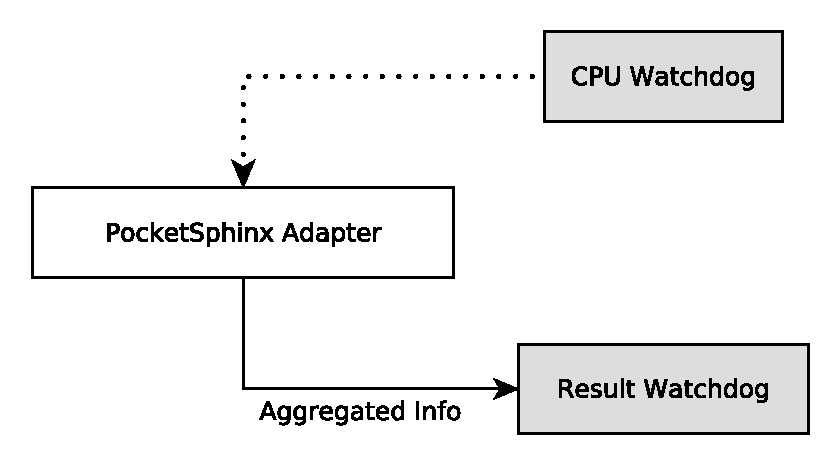
\includegraphics[width=0.66\textwidth]{diagrams/eval_pipeline_1.pdf}
	\caption{Test scenario for existing pipeline}
	\label{pic:eval_p1_diag}
\end{figure}

\begin{figure}[ht]	
	\centering
	\subfloat[Scenario for baseline of proposed pipeline]{
		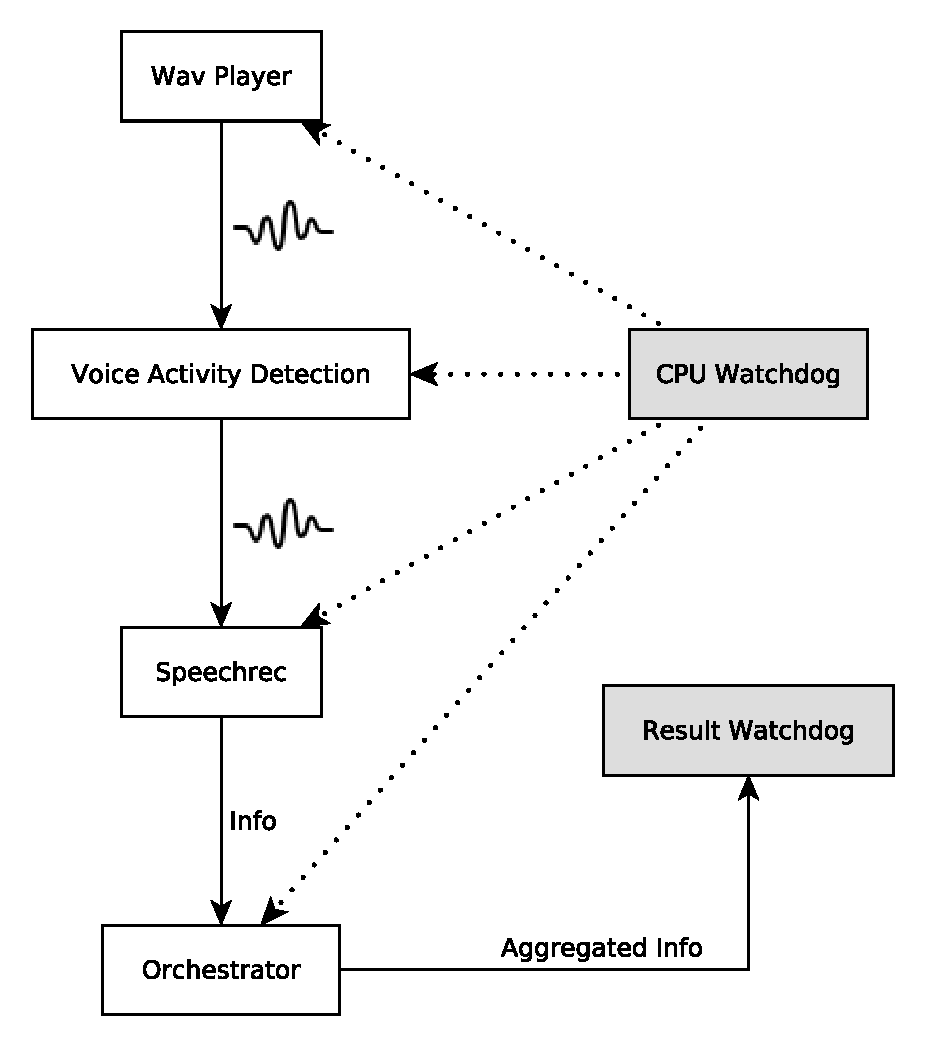
\includegraphics[width=0.5\textwidth]{diagrams/eval_pipeline_2.pdf}
		\label{pic:eval_p2_diag}
	}
	\subfloat[Scenario for elongated baseline of proposed pipeline]{
		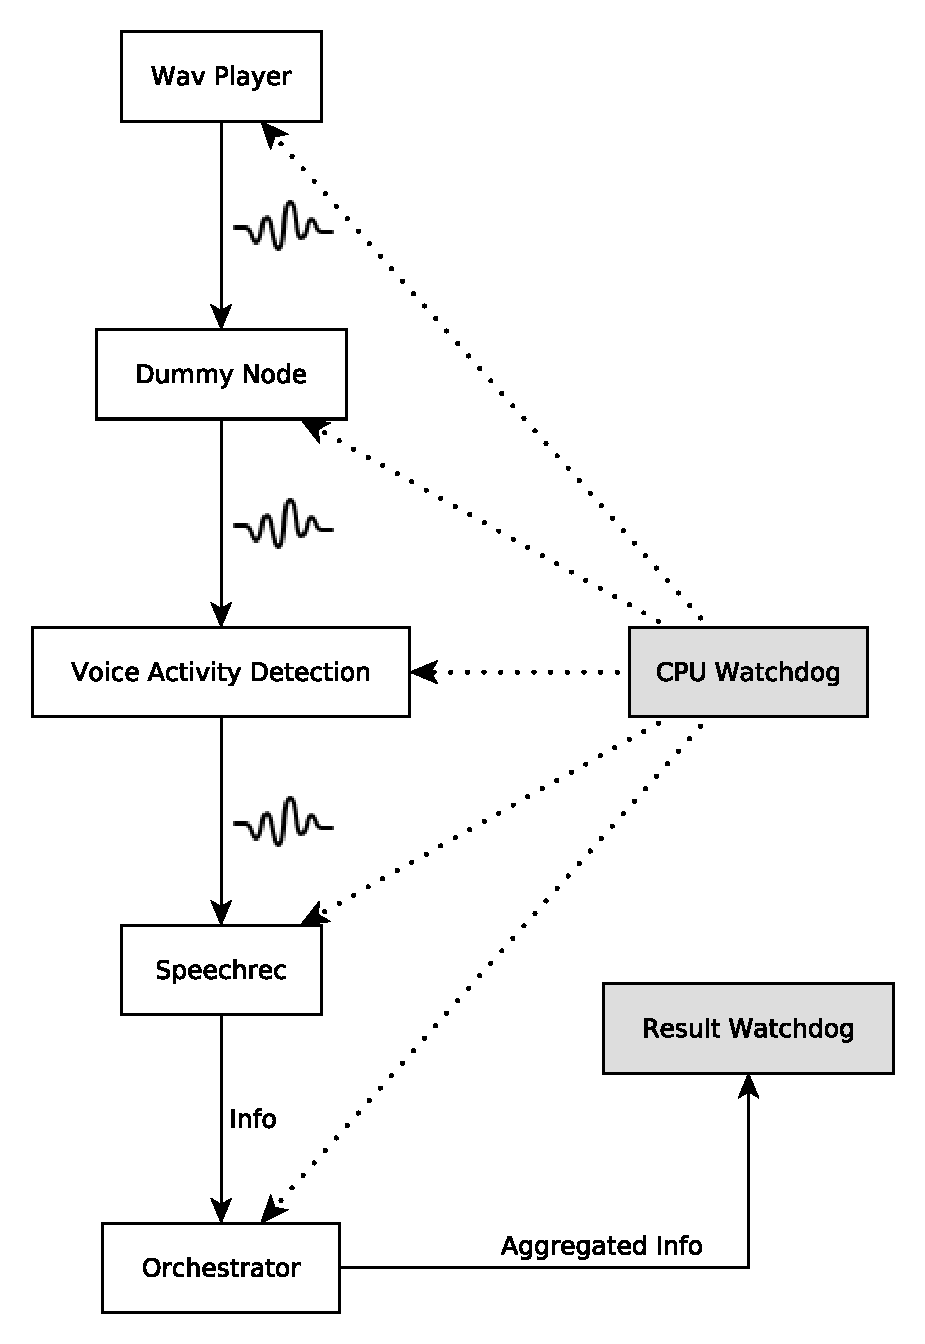
\includegraphics[width=0.5\textwidth]{diagrams/eval_pipeline_4.pdf}
		\label{pic:eval_p4_diag}
	}
	
	\caption{Test scenarios for proposed pipeline}
	\label{pic:eval_p2_4_diag}
\end{figure}


\begin{figure}[ht]	
	\centering
	\subfloat[Test scenario for widened baseline of proposed pipeline]{
		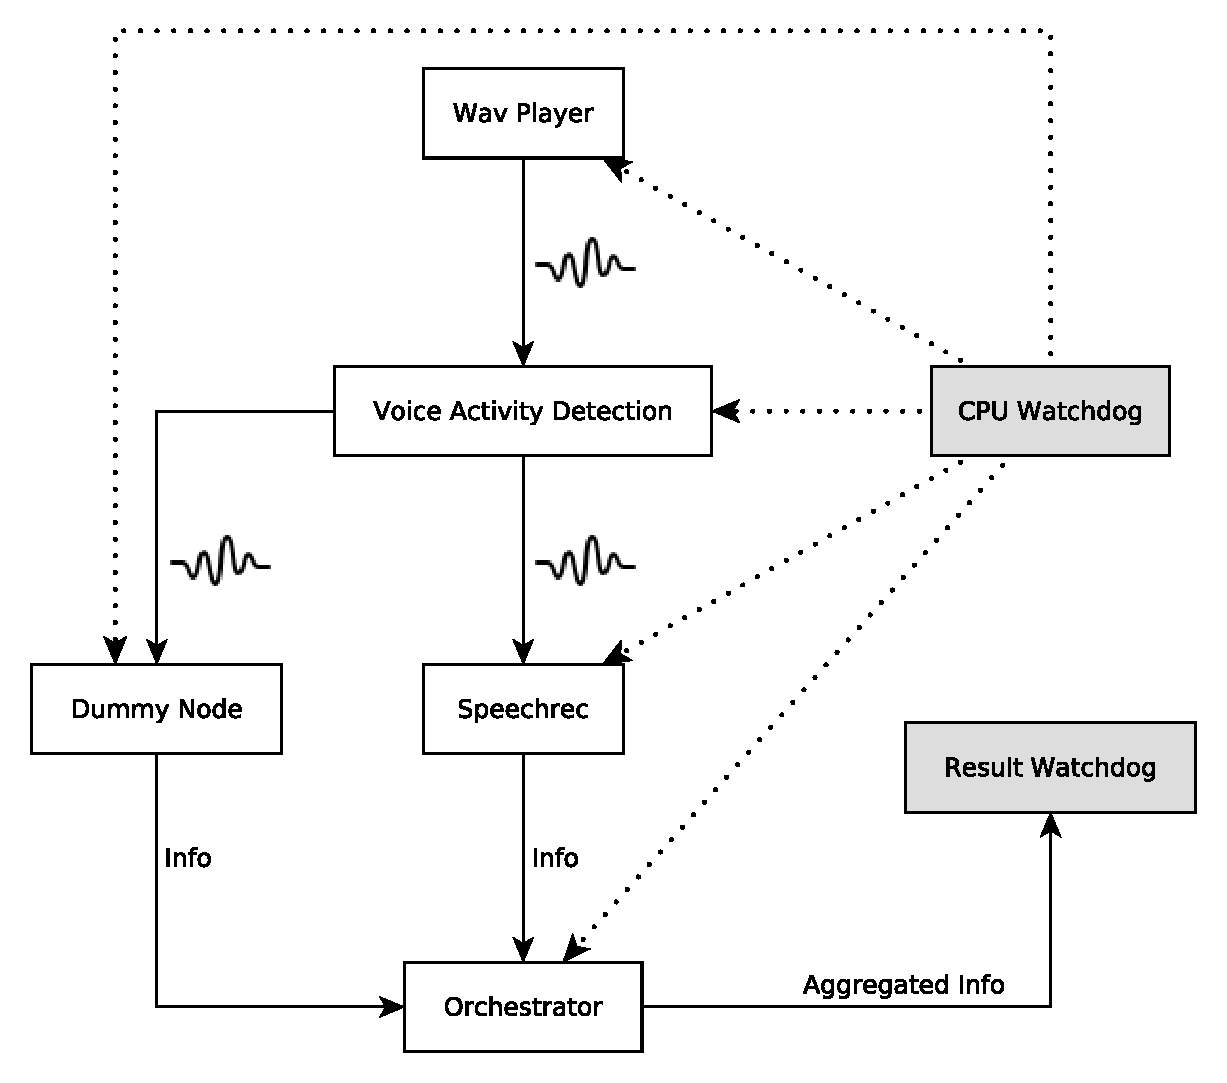
\includegraphics[height=0.4\textwidth]{diagrams/eval_pipeline_3.pdf}
		\label{pic:eval_p3_diag}
	}
	\subfloat[Test scenario for elongated baseline of proposed pipeline]{
		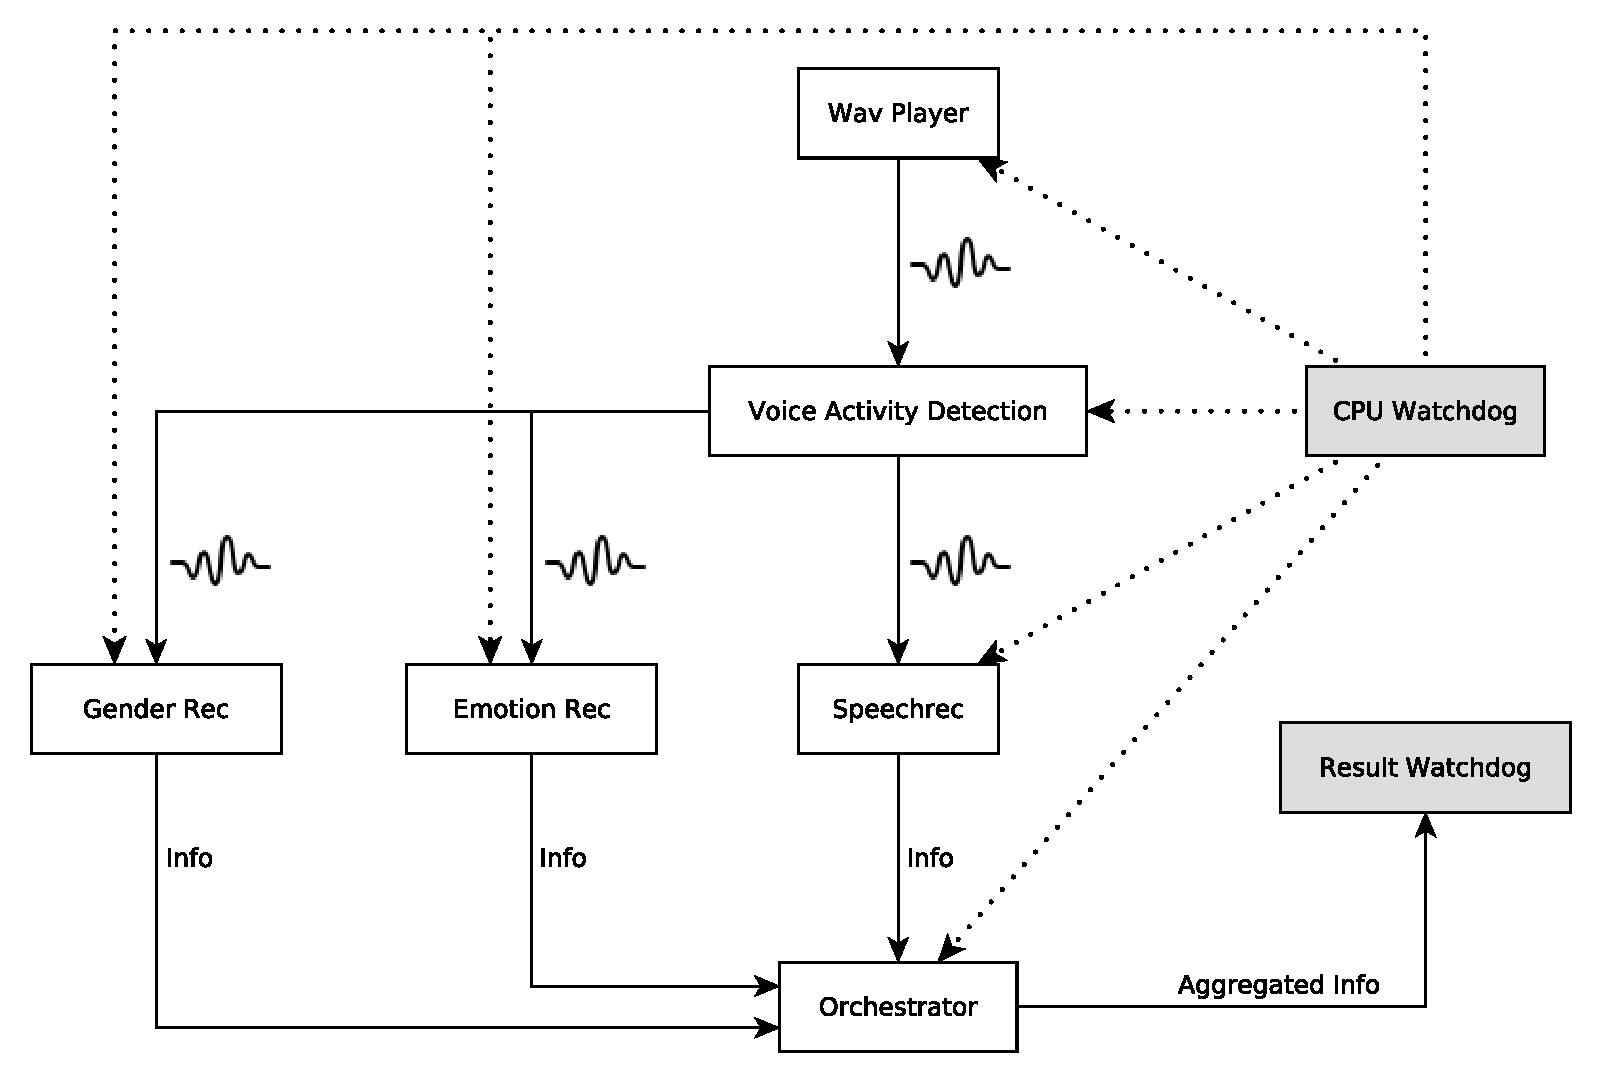
\includegraphics[height=0.4\textwidth]{diagrams/eval_pipeline_5.pdf}
		\label{pic:eval_p5_diag}
	}
	
	\caption{Test scenarios for proposed pipeline}
	\label{pic:eval_p3_5_diag}
\end{figure}

\begin{figure}[ht]
	\begin{tabular}{ | l | p{0.3\textwidth} | p{0.3\textwidth} | p{0.3\textwidth} |}
		\hline
		Pipeline & Correctly recognized sentences & Absolute time till result (in seconds) & CPU time (in CPU seconds) \\ \hline
		Existing & 77.19\% & 1.5596 &  247.44 \\ \hline
		Proposed & 99.77\% & 1.0141 & 1209.3 \\ \hline
		Elongated & 99.77\% & 1.0394 & 1399.63 \\ \hline
		Widened & 99.65\% & 1.0899 & 1665.66 \\ \hline
		Realistic & 99.48\% & 1.7799 & 37517.13 \\ \hline
	\end{tabular}
	\caption{Results of the pipelines in comparison}
	\label{table:eval_dataset_results}
\end{figure}


\subsection{Existing Solution}
Little description:
The existing solution consists only of the PocketSphinxAdapter (PSA), see figure \ref{pic:eval_p1_diag}.
The PSA grabs audio from a microphone using ALSA, filters the audio using an integrated voice activity detection and finally uses, as its name suggests, PocketSphinx to recognize speech.
Recognition results are then communicated via ROS.

Goal: provide a baseline

What can be seen: 

\subsection{Baseline for proposed Pipeline}
Little description:
This configuration of the proposed pipeline is intended to reassemble the PSA as closely as possible.
As seen in figure \ref{pic:eval_p2_diag}, it consists of a voice activity detection, a speech recognizer (using PocketSphinx), the Orchestrator and a Wav file player to feed audio into the pipeline.
Recognition results are gathered by the Orchestrator and then communicated via ROS.

Goal: get additional cost the pipeline itself generates against the existing solution

What can be seen: 

If one compares the results of the pipelines in figure \ref{table:eval_dataset_results}, 
- results for the proposed pipeline are all virtually identical, 


\subsection{Elongated baseline of proposed Pipeline}
This configuration of the proposed pipeline is nearly identical to its baseline, but incorporates a dummy component to evaluate how much overhead in time and CPU cost an additional processing step produces.
As indicated in figure \ref{pic:eval_p4_diag} and by its name, the dummy node does neither alter nor compute information on the audio data it received, but instead just relays it from the WAV player to the VAD.

If one compares the results of the proposed and elongated pipeline in figure \ref{table:eval_dataset_results}, 

Goal: get the overhead in time and cpu cost a single additional component does to the pipeline

What can be seen: overhead cost of adding component is rather small, especially in absolute time needed (2.5 ms), thus negligible

\subsection{Widened baseline of proposed Pipeline}

Goal: get overhead cost of a parallel component

What can be seen: 

\subsection{Realistic version of proposed Pipeline}

Goal: 

What can be seen: 


%----------------------------------------------------------------------------------------------------

\section{Robocup Speech Recognition Test}


\begin{figure}[ht]	
	\centering
	\subfloat[Scenario for baseline of proposed pipeline]{
		\includegraphics[width=0.5\textwidth]{diagrams/robocup_task_t.pdf}
	}
	\subfloat[Scenario for elongated baseline of proposed pipeline]{
		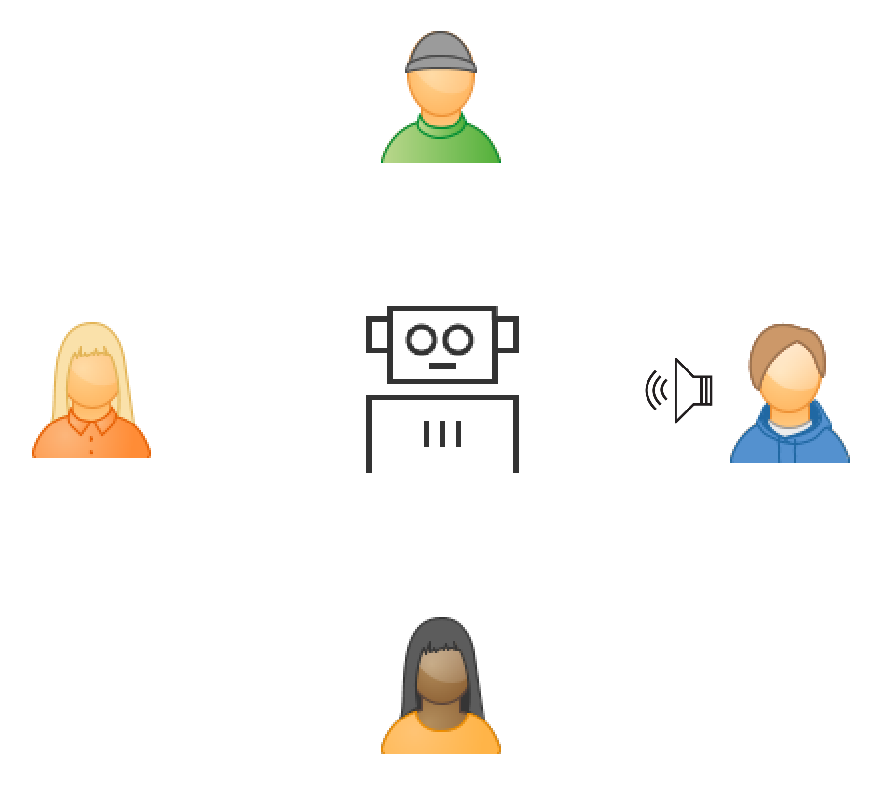
\includegraphics[width=0.5\textwidth]{diagrams/robocup_task_t1.pdf}
	}
	
	\caption{Test scenario for the RoboCup task}
	\label{pic:eval_task}
\end{figure}

\begin{figure}[ht]
	\begin{tabular}{ | l | l | l | l |}
		\hline
		Run & Correctly recognized sentences & Points & Points by SSL \\ \hline
		1 & 50\% & 45 & 0 \\ \hline
		2 & 50\% & 40 & 10 \\ \hline
		4 & 35\% & 25 &  0 \\ \hline
		5 & 40\% & 30 & 10 \\ \hline
		6 & 45\% & 40 & 10 \\ \hline
		7 & 60\% & 50 & 10 \\ \hhline{|=|=|=|=|} 
		Avg & 46.7\% & 38.3 & 6.7 \\
		\hline
	\end{tabular}
	\caption{Results of the existing pipeline in the RoboCup task}
	\label{pic:eval_task_results_old}
\end{figure}

\begin{figure}[ht]
	\begin{tabular}{ | l | l | l | l |}
		\hline
		Run & Correctly recognized sentences & Points & Points by SSL \\ \hline
		1 & 65\% & 50 &  0 \\ \hline
		2 & 55\% & 70 & 20 \\ \hline
		4 & 55\% & 35 &  0 \\ \hline
		5 & 55\% & 50 & 20 \\ \hline
		6 & 60\% & 60 &  0 \\ \hline
		7 & 60\% & 60 & 10 \\ \hhline{|=|=|=|=|} 
		Avg & 58.3\% & 54.2 & 8.3\\
		\hline
	\end{tabular}
	\caption{Results of the proposed pipeline in the RoboCup task}
	\label{pic:eval_task_results_new}
\end{figure}

\begin{itemize}
	\item oftentimes recognition results would be very similar, but once wrong and once right, e.g. ''whats the color of the coke'' would be once interpreted by both pipelines as ''whats the color of the bowl'' and once by the old pipeline as ''whats the color of the fork'' and once correct by the proposed pipeline; other example: sponge was recognized as sausages, thus once wrong
\end{itemize}

